%%=========================================
\section[Bakgrunnsteori]{Bakgrunnsteori}
%%=========================================
\subsection{Smarte hjem}
{\color{red}\emph{Smarte hjem} brukes i denne oppgaven som et samlebegrep for boliger der man kan programmere og styre miljøet, enhetene og apparatene i boligen. Smarte hjem tilbyr funksjonalitet som energieffektivisering, økt komfort, økt sikkerhet, automasjon og generelt enklere bruk. Jeg har valgt å bruke "smarte hjem" i stedet for "smarte hus" for å påpeke at diskusjonen omtaler faste oppholdssteder generelt og ikke bare hus. }

{\color{blue}
Internet of things (iot-oppgaven fra infosik / førprosjektet)

Når hjemmet ditt om noen år tilbyr kontroll over ikke bare lys og temperatur, men garasjeporter, persienner, tv-er, radioer, låsene på døra og statusen til kjøkkenapparater, kan det være en utfordring å tilby gode interaksjonsmetoder.

Fagområde: AmI

Ideén om et smart hjem refererer i følge \citet{peine08} til å bruke informasjons- og kommunikasjonsteknologi (IKT) i hjemmet for å forenkle interoperabilitet av husholdningsprodukter og tjenester. Peine skriver at ideén har vært beskrevet siden 80-tallet og har i de senere år fått en ny interesse i industrien. Faktisk har kontroll av funksjonaliteten i en kontorbygning eksistert siden 70-tallet, med muligheter for å kontrollere lys, varme, elektristet og adgangskontroll fra et sentralt sted. Det tok noen år før man innså at de samme egenskapene kunne være ønskelige å implementere for å automatisere hus. Den sentrale forskjellen mellom et vanlig hus og smart hus er denne muligheten for å styre flere aspekter ved huset gjennom en sentral enhet.

På markedet finnes det nå flere løsninger for å automatisere deler av hjemmet eller tilby gode brukergrensesnitt for å styre funksjonalitet som lys og varme. Disse løsningene bidrar med å ivareta sikkerhet og hjelper til å begrense energiforbruket. De tilbyr gjerne informasjon om hjemmet via en mobilapplikasjon så man kan ha oversikten selv når man er bortreist. Ved å benytte enheter som er tilknyttet internettet, som termostater, lys, låser, sikkerhetssystemer og garasjeporter, kan man styre dem gjennom mobilapplikasjonen\footnote{Et søk i Google på "smarthome" og norske resultater gir for eksempel denne hjemmesiden der en privatperson har tatt i bruk og satt sammen komponenter fra markedet for å skape en helhetlig og gjennomført løsning: http://www.samdal.com/SmartHome.htm}. Disse løsningene er svært praktiske og gir god verdi, men er økt tilgang til informasjon og muligheten til å fjernstyre noen deler av hjemmet det beste vi kan få til i dag?

I en artikkel for Scientific American i 1991 skrev Mark Weiser at de mest dyptgripende teknologiene er de som forsvinner inn i hverdagslivet inntil det er umulig å skille dem ut igjen. Han så for seg at omgivelsene var gjennomtrengt med teknologi for databehandlig og kommunikasjon, og som kunne støtte opp under menneskers liv gjennom såkalt \emph{calm computing} \citet{weiser91}. Dette framtidssynet har styrt utviklingen for forskningsområdene \emph{pervasive/ubiquitous computing} og det peker mot de egenskapene og mulighetene et smart hjem bør tilby. Men hvorfor er ikke smarte hjem smarte nok til å tilby dette framtidssynet ennå? Det har godt mange år og det har blitt gjort mye arbeid siden 1991. Trolig har vi all del-funksjonaliteten som trengs for å implementere dette framtidssynet. Vi har kraftige innebygde enheter, sensorer på størrelse med frimerker, trådløs kommunikasjon, internettet og muligheten til å programmatisk kontrollere elektriske apparater, varme og lys. Vi kan analysere bilder og lydsignaler, gjenkjenne fjes og tale, overvåke og følge brukerenes bevegelser, samt koble oss opp mot eksterne datakilder som værmeldinger og brukerenes kalendere. Grunnen til at vi ikke har disse systemene ennå må være at det er vanskelig å sette det hele sammen og å gjøre god bruk av alle dataene som samles inn. Kunstig intelligens kan være nøkkelen for å gjøre teknologiene vi har om til nyttige tjenester.

For å forstå omgivelsenens tilstand vil det være nødvendig å analysere sensorinformasjon. To lovende input-kanaler er lyd og bilde. Ettersom vi mennesker kommuniserer med tale er det naturlig at et AmI-system skal kunne håndtere dette. Talegjenkjenning er et vanskelig problem, men det er et område det er jobbet mye med opp gjennom årene. Ved bruk av teknikker fra signalprosessering og mønstergjenkjenning kan man identifisere \emph{fonemer} i signalet og deretter ord. Tilsvarende kan man få en datamaskin til å utnytte seg av syn ved å få tak i input som bilder. Disse må også prosesseres og mennesker må gjenkjennes. I følge \citet{augustonugent06} kan datasyn kan være nyttig for å gjenkjenne mønstre i menneskers oppførsel eller oppdage når noe galt har skjedd, som at en eldre beboer har falt. Det kan også brukes til å gjenkjenne gester eller å gjenkjenne fjesuttrykk i et forsøk på å forstå brukerenes følelser. Dersom datasyn skal brukes vil det være viktig å skille beboeren fra besøkende, dyr eller andre bevegelige objekter. Å holde en historie over beboerens siste bevegelser kan hjelpe til med å forstå og avgjøre tilstander. 

Et virkelig smart hjem kan lære av å observere brukere. Teknikker fra maskinlæring, som nevrale nettverk, case-based resonnering og beslutningstrær og støttevektormaskiner er godt utviklet og kan benyttes til dette. Å lære brukernes oppførsel vil være essensielt for at system skal forbedre seg selv over tid, og for å tilby en individuelt tilpasset opplevelse. Forskjellige brukere vil ha forskjellige tilstander, preferanser og vaner, og disse bør tas med i beregningen for at systemet skal være verdifullt.

Data som hentes fra hjemmet kan være interessant for forskjellige brukere, men hvilken informasjon skal hver person motta? Her kommer privathet og sikkerhet inn i bildet. Hvordan og til hvilket tidspunkt tar vi kontakt med brukeren? Uønsket eller unødvendig hjelp er sannsynligvis verre enn ingen hjelp. Påminnelser om oppgaver med lav prioritet kan være frustrerende. Vi ønsker kanskje heller ikke at brukere blir overavhengige av systemet, selv hvis det fungerer godt. For mange brukere kan dette peke mot at vi ønsker et minimalt nivå av hjelp. Dette vil la beboern ta i bruk sin egen kognitive kapasitet og vedlikeholde et høyt nivå av uavhengighet. 

Ettersom vi snakker om hvorfor og hvordan man vil utvikle løsninger for å skape smarte hjem kan det være en god idé å ha kontakt med brukermassen. Smarte hjem er et relativt nytt produkt for det store markedet, så det er ikke sikkert at brukerene vet hva de vil ha fra et smart hjem, eller om de vil ha et smart hjem i det hele tatt. Men ettersom dette kan sees på som utviklingen av et nytt produkt vil det allikevel være klokt å ta pulsen på framtidige kunder. I stedet for å dytte behov på brukeren kan det være bedre å støtte opp under brukerens faktiske behov. Dette kan hjelpe oss å bygge produkter som blir godt motatt og dermed kan vi framskynde innføringen av smarte og automatiserte hjem.

\citet{bonino11} ledet en interessant italiensk studie som spurte en gruppe hva de ville spurt hjemmet sitt dersom det var intelligent. Studien viser at folk flest har sterke følelser knyttet til hjemmet. Det er et trygt og koselig sted. Det er et sted til å stole på og følelsen av å returnere dit er god. Generelt er å føle seg bra en del av hjemopplevelsen. Atmosfæren er behagelig og tilpasset brukerens preferanser og folk liker at de kan gjøre hva de selv vil. Brukere har følelsen av å være i kontroll.

Artikkelen presenterer hva gruppen mener er de viktigste områdene for det smarte hjemmet:
\begin{itemize}
  \item Intelligente brukergrensesnitt på hvitevarer, for eksempel stemmekontrollerte oppvaskmaskiner.
  \item En tilgjengelig klokke, for planlegging av aktiviteter.
  \item Tilgang til værinformasjon, da ønskede fritidsaktiviteter ofte avhenger av været utendørs.
  \item Ivaretagelse av egen sikkerhet og husets sikkerhet. Innbruddsbeskyttelse og automatisk oppdagelse av farer, som røyk-, varme- eller gassutvikling.
  \item Informasjon om energiforbruk og forslag til hvordan energiforbruket kan reduseres.
  \item Kontroll av husets underholdningssenter.
  \item Tilgjengelig kommunikasjonsbehov som å lese epost og bruke telefon.
  \item Automatisk oppdagelse og eventuell reparasjon av problemer.
  \item Husholdningsoppgaver som hjelp med oppgaver til å holde huset rent og komfortabelt, håndtering av mat og hjelp med planlegging av innkjøp.
  \item Komfortrelaterte problemer som lysregulering, temperaturregulering og operering av vinduer og persienner.
  \item Personlig assistanse, som å be huset om hjelp til å huske ting, søke opp informasjon og håndtere andre dagligdagse oppgaver.
\end{itemize}

En annen studie av brukerbehovene for smarte hjem presenteres av \citet{userreq}. Her omtales en empirisk studie utført på seks forskjellige steder i fem europeiske nasjoner. Studien bruker en scenario-drevet tilnærming og brukte kvantitative og kvalitative metoder for å få tilbakemelding fra brukermassen om konsepter innen smarte hjem. Deltakerene kom opp med en rekke forslag og ideer til hva et smart hjem bør tilby og prioriteringsrekkefølgen for disse funksjonalitetene. Generelt ble det funnet godt med beviser på hva brukere er interessert i: Systemet skal være lett å bruke og å konfigurere. Det skal ikke kreves programmering eller vedlikehold av noe slag. Systemet skal være modulært og tilby å justere for individuelle preferanser. Alle deltakerene var enig om at personvernet ikke måtte brytes gjennom overvåking. Den følgende listen er sortert med høyeste prioritet først.
\begin{enumerate}
  \item Brukeren må alltid være i kontroll av systemet.
  \item Systemet må ivareta sikkerhet, og beskytte personvernet.
  \item Et nytt system må gi ny verdi over eksisterende systemer.
  \item Systemet må ikke unødvendig overta rollen til direkte kommunikasjon mellom mennesker.
  \item Hjemmekomforten skal alltid ivaretas.
  \item Systemet skal tilby passende informasjon til passende brukere på forskjellige lokasjoner basert på brukerpreferanser.
  \item System skal redusere tiden som trengs for å utføre husholdningsoppgaver som vasking.
  \item Systemet skal integrere og kombinere funksjonaliteten til hvitevarer.
  \item Systemet skal være energibesparende.
  \item Systemet skal være kostnadsbesparende.
  \item Systemet skal støtte organiseringsaktiviteter og planlegging for flere personer i hjemmet, mellom forskjellige hjem og mellom hjemmet og jobb.
  \item Systemet skal tilby adgangskontroll og respektere individuelle preferanser og autoriteter.
  \item Systemet skal holde informasjon om kontekst og omgivelsene.
  \item Systemet skal forholde seg til implisitte sosiale normer.
\end{enumerate}

Basert på denne forskningen bør vi lete etter programvare som gjør det enkelt å automatisere, å se hjemmets status og å gi hjemmet kommandoer. Det hele må gjøres med sikkerhet og bevarelse av personvernet. Dette peker mot at programvare og data , i hvert fall delvis, må holdes lokalt.
}

{\color{blue}
Smarte hjem ønsker å tilby funksjonalitet relatert til gevinst innen økonomi og komfort, som at lys og varme skrues av og på automatisk avhengig av beboernes tilstedeværelse. Men det kan argumenteres for at den viktigste funksjonaliteten er for å forbedre en uavhengig livsstil for eldre og funksjonshemmede. Basert på antallet artikler om teamet må å opprette støtte for at eldre og funksjonshemmede skal få leve uavhengig i lengre tid være en av de mest studerte tilnærmingene til smarte hjem. En god grunn er at dette er den gruppen mennesker som vil ha størst nytte av et smart hjem. Muligheten til å fortsette å leve uavhengig og selvstendig i sitt eget hjem, framfor å bli innlagt på en institusjon, er virkelig verdifull. Et smart hjem kan hjelpe til med funksjonalitet som å gi påminnelser om at medisin må tas og å oppdage dersom noe har gått galt og automatisk ta kontakt med hjelpetjenester eller familie.

Den andre gode grunnen til at denne tilnærmingen studeres mye er på grunn restriksjonene denne beboergruppen har i sitt levesett. Når de forskjellige aktivitetene beboerne utfører kan telles på noen få hender blir det store problemet om å få et datasystem til å forstå menneskelige aktiviteter mye enklere. Det blir satt restriksjoner på problemet som gjør at det faktisk kan løses. Å løse problemet uten restriksjoner kan vise seg å være en svært vanskelig og kanskje umulig oppgave. Vi mennesker gjør ofte flere aktiviteter på en gang, samarbeider med andre mennesker og vi kan avslutte aktiviteter midtveis.

\citet{desilva12} påpeker at for systemene som fokuserer på støtte av eldre og funksjonshemmede er det ekstra viktig å detektere mennesker, ettersom en av hovedfunksjonalitetene til et slikt system er å gjenkjenne hvilken tilstand beboeren er i. Dersom beboeren for eksempel har falt er det viktig å gjenkjenne objektet på bakken som et menneske og ikke som en livløs gjenstand. Ettersom å gjenkjenne mennesker er av høyeste prioritet benytter mange av prosjektene i denne kategorien videoovervåkning. Når det gjelder deteksjon av fall skriver \citet{elliot09} om bruken av en pendel, refleksjons-sensorer og et nevralt nettverk for å følge pendelens posisjon i reell-tid. Resultatene indikerte at teknikken er tilstrekkelig sensitiv og kan brukes til å gjenkjenne forskjellene mellom en person som finner balansen og en som er i ferd med å falle. På denne måten kan hjemmet gjenkjenne og potensielt forhindre et fall før det skjer.

Casattenta-prosjektet gjør bruk av utplasserte sensorer, \emph{monitoring nodes}, fordelt i hjemomgivelsene, samt bærbare enheter, \emph{active keys}, for å overvåke beboernes helse og aktivitet (se figur \ref{casattenta}). \citet{casattenta} skriver at målet er å tilby tilstrekkelig, men ikke-påtrengende, overvåkning for å forbedre sikkerheten og livskvaliteten til eldre mennesker som bor alene. Omgivelsessensorene tillater overvåking av de typiske funksjonene i et avansert hjem: tilgangskontroll, gasslekkasjer, lys, lyd, åpne vinduer, fuktighet og temperatur. Interaksjonen mellom de utplasserte sensorene og de bærbare enhetene tillater innendørs sporing av menneskene og muligheten til å oppdage farlige hendelser. Sporingen realiseres ved å benytte signalstyrken mellom den bærbare enheten og sensorene i omgivelsene. Prosjektet gjorde bruk av den strømgjerrige ZigBee-protokollen for kommunikasjon mellom enhetene. Systemet kan også oppdage om uautoriserte personer befinner seg i hjemmet. Dersom en person oppdages ved en infrarød sensor og systemet ikke registrerer en bærbar enhet i det samme området kan en alarm aktiveres. Alarmen kan få brukerens bærbare enhet til å vibrere eller aktivere et web-kamera i nærheten for å tilby informasjon til slektninger eller andre. Systemet kan også detektere fall ved kombinasjonen av et akselerometer i den bærbare sensoren som kan si om personen ligger, og sporingen som kan si om personen befinner seg på soverommet eller ikke. Dersom et fall registreres kan systemet vibrere den bærbare enheten. Dersom brukeren ikke stopper alarmen går den videre og systemet tar kontakt med utenforstående og skrur på web-kamera for å tilby innsyn til hjemmet.

I disse dager dukker energibesparing stadig opp i den offentlige debatten. Å kutte energiforbruket er et samlet mål for mange i vår del av verden. Dette strekker seg også til hjemmet og kan blant annet oppnås ved å skru av lys og varme når det ikke trengs. Et smart hjem kan enten aktivt gå inn og skru ned eller av lys, varme og apparater når de ikke er i bruk, eller det kan overvåke energibruken og periodisk komme med forslag til forandring i brukerens holdning til bruk av elektrisitet. Et alternativ for å oppnå bedret energieffektivitet er å anvende multiagent-paradigmet og gi agentene et mål om å være energieffektive.

I kapittel to så vi på kunstig intelligens' definisjon av agenter og hvordan denne tilnærmingen kan hjelpe oss å løse problemer. Noen problemer er svært vanskelige eller umulige for en enkelt agent å løse. Her kan et multiagent-system komme inn i bildet. Dersom hjemmet er kontrollert av en gruppe agenter med forskjellige egenskaper og ansvarsområder kan de sammen potensielt løse kompliserte problemer. Nye problemer innen kommunikasjon, prioriteringer og utførelse dukker opp, men dersom disse totalt sett er enklere å løse er tilnærmingen alt i alt god. Agentene i et multiagent-system er som regel uavhengige og fokuserer på seg selv og sin oppgave. Systemet som en helhet er desentralisert og hver agent kjenner ikke til hele problemområdet. Det er derfor viktig at kommunikasjonen er god for å effektivt kunne løse problemer. En stor fordel med et slikt system er fleksibiliteten. Ettersom det er desentralisert kan nye agenter legges til og systemet som en helhet kan modifiseres uten større problemer. Dette gjør også at systemet er enklere å vedlikeholde og at det selv kan håndtere eventuelle problemer. Flere agenter som kan håndtere de samme oppgavene kan leve i systemet slik at dersom en av dem feiler håndterer den andre fremdeles oppgaven. Flere prosjekter i litteraturen har angrepet smarte hjem-problemet med multiagent-paradigmet. Jeg har lyst til å nevne to prosjekter i noe detalj.

MavHome-prosjektet (Managing An Intelligent Versatile Home) har hatt som mål å skape et hjem som oppfører seg som en rasjonell agent. \citet{mavhome} skriver at agenten forsøker å oppnå to mål samtidig: å maksimere beboernes komfort og å minimere kostandene for å operere hjemmet. For å nå disse målene må agenten ha evnen til å forutse bevegelsesmønstrene og bruken av elektriske enheter blant brukerene. Individuelle agenter kan ta seg av en del av problemet, men må koordinere deres handlinger for å oppnå det overordnede målet.

Med \emph{Thinkhome}-prosjektet påpeker \citet{thinkhome} at tidligere løsninger på smarte hjem ikke har klart å holde energinivået lavt og samtidig tilbudt god komfort for beboerne. Thinkhome benytter en stor kunnskapsbase for å ta vare på den nødvendige informasjonen for energieffektivitet og brukerkomfort, og anvender multiagent-paradigmet for å bygge et intelligent system. På samme måte som MavHome fokuserer Thinkhome på energibruk på grunnlag av økonomiske og bærekraftige mål. Samtidig prioriteres komfort ettersom nettopp dette er høyt rangert blant brukerbehovene i et automatisert hjem. Målet for prosjektet er danne en arkitektur som kan brukes i neste generasjons bygninger.

De fleste av oss har tilgang til en såkalt personlig assistent på smarttelefonen. På Android (og gjennom nettlesere) har man \emph{Google Now} og på iOS har man Apple's \emph{Siri}. Begge produktene er intelligente, personlige assistenter som tilbyr et brukergrensesnitt for naturlig språk hvor man kan få svar på spørsmål, anbefalinger og utførelser av handlinger gjennom web-tjenester. Begge tilpasser seg brukeren over tid og forsøker å levere individuelt tilpassede resultater.

I januar 2014 presenterte Intel et headset som i framtiden skal utfordre de personlige assistente fra Apple og Google, og de kaller det \emph{Jarvis}\footnote{http://www.theinquirer.net/inquirer/news/2325465/intels-jarvis-headset-will-take-on-apples-siri-and-google-glass-by-working-offline, hentet des 2014.}. Intel's fordel vil være at talegjenkjenningen utføres i headsettet, på den nye \emph{Edison-modulen}\footnote{http://www.intel.com/content/www/us/en/do-it-yourself/edison.html, hentet des 2014.}. Dermed fungerer den personlige assistenten selv når man ikke har kontakt med internettet. Når man kan unngå å sende forespørselen på en rundtur over nettet, for prosessering og analyse et annet sted, spares det mye tid og man unngår forsinkelsen som gjør dagens eksisterende systemer vanskelige å bruke. Science fiction inspirer ofte teknologisk utvikling og Intel's valg av navn er en klar referanse til datasystemet \emph{J.A.R.V.I.S.} fra \emph{Iron Man-filmene}\footnote{http://marvel-movies.wikia.com/wiki/J.A.R.V.I.S., hentet des 2014.}. Dette programmet styrer heltens smart hjem og kontrollerer alt der, som innemiljø og sikkerhet. Samtidig fungerer det som en personlig assistent og tilbyr hjelp med informasjonsgjenfinning og planlegging. Systemet interageres med gjennom touch-skjermer, talegjenkjenning, syntesert tale, holografi og robotikk. Så hvordan kan en slik personlig assistent som ikke bare tilbyr informasjon, men som selv utfører avanserte oppgaver, implementeres?

Mange webtjenester som folk flest bruker i dag, som kalendere, værkilder og trafikkdata, tilbyr også muligheten til å spørre kildene programmatisk gjennom API'er (\emph{application programming interfaces}. Dermed kan det smarte hjemmet kombinere sensordata fra huset med webtjenester. Basert på data fra kalendere, vær, trafikk og brukerens preferanser kan det smarte hjemmet for eksempel kalkulere at brukeren har tid til å gå til sitt første møte for dagen. Dersom brukeren svarer bekreftende på et slikt forslag kan systemet planlegge reiseruten til møtestedet og laste ned nødvendige kartdata til brukerens mobiltelefon. Dette er funksjonalitet som kan implementeres i dag. Et mer avansert scenario, der hjemmet gjør større, proaktive handlinger på brukerens vegne, og har muligheten for å hente informasjon fra informasjonskilder brukeren ikke kjenner til krever en annen teknologi. Dette er teknologi som eksisterer, men ennå ikke er utbredt. \citet{semantic01} legger grunnlaget for det neste steget i webbens evolusjon, en semantiske web. Dersom hjemmet for eksempel skal kunne kjøpe ønskede billetter på brukerens vegne trengs det en felles, vidspredt platform for kunnskapsrepresentasjon og en felles forståelse for beskrivelsen av og sammenhengene mellom informasjon. Først da kan systemer kommunisere seg i mellom uten menneskelig intervensjon på en trygg og sikker måte. En semantisk web foreslår \emph{Resource Description Framework (RDF)} for å representere kunnskap og avtalte ontologier for å beskrive informasjon og sammenhenger. At data er lagret i RDF gjør det enkelt å ta kontakt med mange forskjellige datakilder samtidig og lage kompliserte spørringer. Ontologiene gjør at det oppnås en felles forståelse for hvordan kunnskap henger sammen. Modellen som en helhet klargjør for å lage automatiserte agenter som kan kommunisere seg i mellom og utføre arbeid og transaksjoner som tidligere trengte sterk menneskelig innblanding, som å ta kontakt med en selgeragent hos en billettjeneste og bestille billetter på brukerens vegne.

Video gir potensialet for å realisere virkelig smarte systemer som kan motta kommandoer gjennom gester, forstå hjemmets tilstand, gjenkjenne beboerenes aktiviteter og kanskje til forstå kontekst. Video produserer store datamengder og dette gir en større teknisk utfordring med henhold til lagringsplass og datautvinning enn bruk av enklere sensorer. Heldigvis er det utviklet mange gode teknikker for å analysere bilder og desto mer tid som går desto større blir lagringskapasitetene våre.

Et eksempelprosjekt som blant annet gjør bruk av video er \emph{Placelab-prosjektet}, beskrevet av \citet{placelab05}. I sin studie gjorde de blant annet bruk av ni infrarøde kameraer, ni fargekameraer og atten mikrofoner spredd gjennom en leilighet. Ved bruk av bildebehandlingsalgortimer kunne de velge hvilke av datastrømmene som best fanget beboerens oppførsel til et gitt tidspunkt.
Desverre er bruken av kameraer et problem i hjemmescenariet.

{\color{red} Ref og ref} har vist at brukere har sterke motsetninger mot overvåking i sitt eget hjem. Selv dersom det kan garanteres at dataene fra kameraene holdes lokalt kan følelsen av at personvernet er utsatt være nok til at brukerene vil holde seg unna. Baksiden av videomedaljen er beskyttelse av personvernet og brukerenes følelse av å opprettholde et privatliv i hjemmet. Intuitivt kan man forestille seg at de færreste brukere i utgangspunktet ønsker kameraer som filmer dem overalt i hjemmet. Selv dersom det kunne garanteres at informasjonen aldri forlot hjemmet, eller at den kun blir lagret i en kort tidsperiode, vil tilsynelatende konstant overvåking være noe mange vil sette et stort spørsmåltegn ved. I overvåkningssamfunnet i George Orwell's \emph{1984} har hver leilighet en skjerm med tilhørende kameraovervåking som kan se stort sett alt som foregår. I dette samfunnet har befolkningen over tid godtatt overvåkningen, i den tro at det er til deres eget beste. I vår verden ser ut til at folk flest godtar dagens nivå av overvåkning gjennom loggførte posisjonsdata fra smarttelefoner, søkeord og forflytninger med fly og bil. Men introduksjonen av videokameraer i stuene vil kanskje oppleves som for mye, selv hvis informasjonen kun holdes og brukes lokalt.
}

\subsection{Maskinlæring}
{\color{blue}
Prosjekter som benytter maskinlæring for å forstå input. Maskinlæring i forbindelse med smarte hjem. Teori klassifisering.

La oss begynne med en definisjon på maskinlæring fra Arthur Samuel (1959): "Maskinlæring gir datamaskiner evnen til å lære uten å bli eksplisitt programmert."

Denne definisjonen er over 50 år gammel, men den fanger hva vi er ute etter. Vi er interessert i å få datamaskinene til å lære å gjøre nyttige ting uten å behøve å fortelle dem eksplisitt hvordan hver enkelt oppgave skal utføres. Dette er nødvendig da det med mye og kompleks data raskt blir umulig for en programmerer å beskrive alle deloppgavene som må utføres.

Alle maskinlæringsproblemer kan konseptualiseres som å finne en funksjon som knytter input til output. Målet kan være å tilnærme en enkel matematisk funksjon, det kan være å spå aksjekursen basert på historisk data eller det kan være å gi sannsynligheten for et en epost er spam, basert på innholdet. Man tar erfaring, i form av empirisk data, og kjører det gjennom en algoritme som forsøker å finne en funksjon som dekker denne kunnskapen best mulig.

I dette prosjektet skal dataene en gest danner knyttes til navnet på en gest. Dette er en form for maskinlæring kalt overvåket læring. Målet er å klassifisere nye data korrekt, basert på treningsgrunnlaget fra tidligere data. Læringen sies å være overvåket fordi vi bidrar med informasjon om hvilke klasser som hører til hvilke data i treningseksemplene. Framgangsmåten er å mate maskinen med mange eksempler på denne koblingen mellom data og gest og håpe at maskinen finner en matematisk funksjon som tilnærmer denne sammenhengen godt.

Dataene vi jobber med i dette prosjektet har 128 egenskaper og 50 treningseksempler av hver klasse. Dette er relativt mange egenskaper og få treningseksempler. Basert på disse karakteristikkene er det sannsynlig at enkle, lineære modeller vil gi de beste resultatene {\color{red} refeefer! Scikitlearn?}. Mer avanserte klassifiseringsteknikker, som for eksempel nevrale nettverk, kan i teorien tilnærme enhver funksjon, men de trenger langt flere treningseksempler for å finne de sanne sammenhengene mellom datapunktene.

Vi mater et treningssett av datapunkter til en valgt læringsalgoritme. Algoritmen danner seg en hypotese om hva slags modell som best beskriver dataene. Denne hypotesen kan så benyttes til å gjøre gjetninger på nye datapunkter. Hypotesen avhenger av egenskapene i datapunktene. I en lineær modell er hypotesen en funksjon av egenskapene $x$ i treningsdataene, der hver egenskap blir vektet av $\theta$-verdier:

\begin{equation}
h_\theta(x) = \theta_0x_0 + \theta_1x_1 + \theta_2x_2 + ... + \theta_nx_n
\label{eq:hypotese-lin}
\end{equation}

I dette prosjektet har hvert datapunkt $n = 128$ egenskaper. La oss modellere $x$ til å være en vektor med disse egenskapene: 
\[
x =
\begin{bmatrix}
x_0 \\
x_1 \\
x_2 \\
.. \\
x_{128}
\end{bmatrix}
\in R^{128},
\]
Vi lar $\theta$ være en tilsvarende vektor: 
\[
\theta =
\begin{bmatrix}
\theta_0 \\
\theta_1 \\
\theta_2 \\
.. \\
\theta_{128}
\end{bmatrix}
\in R^{128}
\]

Dersom vi nå tar den transponerte av $\theta$ og lar \(x_0 = 1\), kan vi i stedet for (\ref{eq:hypotese-lin}) skrive hypotesen elegant og kompakt som indreproduktet av vektorene:
\begin{equation}
h_\theta(x) = \theta^{T}x
\label{eq:hypotese-kompakt}
\end{equation}

En vellykket hypotese vekter $\theta$-verdiene slik at algoritmen gir de beste mulige resultatene. Denne vekttingen tilsvarer det å finne hvilke egenskaper i dataene som er de viktigste for å angi hvilken klasse dataeksempelet tilhører. Så hvordan velger man disse $\theta$-verdiene? Vi ønsker $\theta$-verdier slik at hypotesen \(h_\theta(x)\) er nære klassen $y$, for treningseksemplene \((x,y)\). Treningseksemplene  \((x,y)\) representerer eksempelkoblinger mellom data og klasse. Dersom vi antar at hypotesen er en lineær funksjon og at dataene kun har to egenskaper, kan vi plotte hypotesen som en linje gjennom datapunktene. For hvert nye treningseksempel algoritmen prosesserer vil $\theta$-verdiene justeres og linjen vil tilpasses til å følge datapunktene som angir en av de to klassene bedre. Etter at funksjonen er trent på en rekke treningseksempler vil linjen forhåpentligvis danne et klart skille mellom datapunktene som utgir de to klassene (se figur \ref{figure:separator}).

\begin{figure}[h!]
\centering
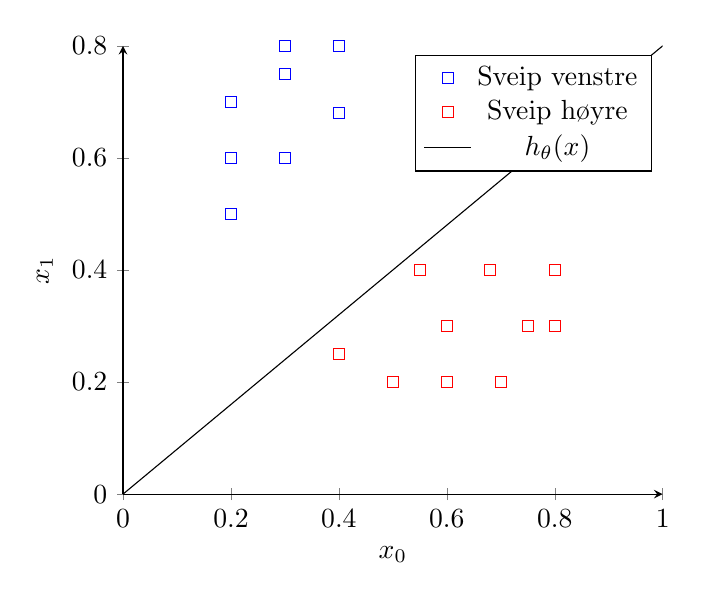
\begin{tikzpicture}
\begin{axis}[
    axis lines = left,
    xlabel = $x_0$,
    ylabel = {$x_1$},
]
\addplot[
    only marks,
    color=blue,
    mark=square,
    ]
    coordinates {
    (0.2,0.7)(0.2,0.5)(0.2,0.6)(0.3,0.8)(0.3,0.6)(0.3,0.75)(0.4,0.8)(0.4,0.68)
    };
\addlegendentry{Sveip venstre}
\addplot[
    only marks,
    color=red,
    mark=square,
    ]
    coordinates {
    (0.55,0.4)(0.4,0.25)(0.7,0.2)(0.5,0.2)(0.6,0.2)(0.8,0.3)(0.6,0.3)(0.75,0.3)(0.8,0.4)(0.68,0.4)
    };
\addlegendentry{Sveip høyre}
\addplot [
    domain=0:1, 
    samples=100, 
    color=black,
]
{0.8*x};
\addlegendentry{\(h_\theta(x)\)}
\end{axis}
\end{tikzpicture}
\caption{Plot av en lineær hypotese som deler datapunktene i to tilhørende klasser.}
\label{figure:separator}
\end{figure}

Separatoren i figur \ref{figure:separator} er en linje i to dimensjoner. En separator i tre dimensjoner vil danne et plan. Det blir deretter vanskelig for oss å forestille oss en separator som opererer i mer enn tre dimensjoner. Heldigvis kommer matematikken til vår hjelp da den ikke bryr seg om våre visuelle begrensninger og fungerer like godt i 128 dimensjoner som i tre. Vi har konkludert med at en lineær modell bør få sjansen til å skille dataeksemplene våre, men hvilken algoritme bør vi benytte? To lignende, mye brukte og robuste teknikker er logistisk regresjon og støttevektormaskiner.

\subsubsection**{Logistisk regresjon}
I logistisk regresjon modelleres sannsynlighetene som beskriver ulike utfall av en logistisk sigmoid-funksjon. Denne funksjonen tar en hvilken som helst input-verdi og gir en output-verdi i området \([0,1]\). Figur \ref{figure:sigmoid} viser den generelle sigmoid-funksjonen. Vi ser at ved større positive x-verdier gir funksjonen et resultat nære 1, mens for større negative verdier gir funksjonen et resultat nære 0.

\begin{equation}
g(x) = \frac{1}{1 + e^{-x}}
\label{eq:sigmoid}
\end{equation}

\begin{figure}[h!]
\centering
\begin{tikzpicture}
\begin{axis}[
    axis lines = center,
    xlabel = $x$,
    ylabel = {$y$},
]
\addplot [
    domain=-5:5, 
    samples=100, 
    color=red,
]
{1 / (1 + e^(-x))};
%\addlegendentry{\(g(x) = \frac{1}{1 + e^{-x}}\)}
\end{axis}
\end{tikzpicture}
\caption{Plot av en ordinær sigmoidfunksjon.}
\label{figure:sigmoid}
\end{figure}

La oss si vi har to mulige klasser, \(y \in \{0,1\}\). Hvis \( h_\theta(x) \geq  0.5\), gjetter vi at klassen \(y = 1\). Hvis \( h_\theta(x) < 0.5\), gjetter vi \(y = 0\).

Når vi nå kombinerer (\ref{eq:hypotese-kompakt}) og (\ref{eq:sigmoid}) får vi den logistiske hypotesen (\ref{eq:logistic}).

\begin{equation}
h_\theta(x) = \frac{1}{1 + e^{-\theta^{T}x}}
\label{eq:logistic}
\end{equation}

Igjen representerer $\theta$ vektingen av egenskapene $x$ i treningsdataene. (\ref{eq:cost}) viser formelen for logistisk regresjon.

\begin{equation}
J(\theta) = 
    \frac{1}{m} \sum_{i=1}^{m} cost(h_\theta(x^{(i)}), y)
\label{eq:cost}
\end{equation}

Vi ser at $J(\theta)$ er et gjennomsnitt av en kostnadsfunksjon, definert av hypotesen til hvert treningseksempel og den tilhørende korrekte klassen. Kostnadsfunksjonen (\ref{eq:costdetail}) er definert med delt forskrift slik at kostnaden er 0 dersom klassen er 1 og hypotesen er 1, men dersom klassen er 1 og hypotesen går mot 0, går kostnaden mot uendelig. Den delte forskriften gjør at det samme gjelder for det motsatte tilfellet, der kostnaden er lav dersom klassen er 0 og hypotesen gjetter 0, men øker mot uendelig dersom hypotesen går mot 1.

\begin{equation}
    cost(h_\theta(x^{(i)}), y) = \begin{cases}
    -log(h_\theta(x)), & \text{hvis $y=1$}.\\
    -log(1-h_\theta(x), & \text{hvis $y=0$}.
  \end{cases}
  \label{eq:costdetail}
\end{equation}

For å tilpasse $\theta$-verdiene er strategien å minimere kostnadsfunksjonen (\ref{eq:costdetail}). Dette gjøres ved å benytte en oppdateringsregel. Regelen oppdaterer egenskapsvektoren $\theta$ ved å trekke fra resultatet fra den partiellderiverte av kostnadsfunksjonen, dempet av en faktor $\alpha$ (\ref{eq:gradient}).

\begin{equation}
\theta_j \leftarrow \theta_j - \alpha \frac{\delta}{\delta\theta_j}J(\theta)
\label{eq:gradient}
\end{equation}

Ettersom den deriverte i et gitt punkt kan sees på som brattheten til kurven i det punktet vil denne oppdateringen tilsvare å stadig ta mindre steg i den retningen som fører mot en lavere verdi på kurven. På en to-dimensjonell graf vil det si å følge plottet nedover mot et bunnpunkt, men algoritmen fungerer på samme vis i høyere dimensjoner. Denne oppdateringsregelen kalles "gradient descent" og brukes i flere maskinlærings-sammenhenger for å finne minimumsverdier.

Etter at $\theta$-verdiene er tilpasset av treningsdata kan modellen gjette hvilken klasse et nytt datapunkt tilhører ved p benytte (\ref{eq:logistic}). For å lære å skille mellom de 10 ulike klassene benyttes strategien "en-mot-resten". For hver klasse trenes det en egen hypotese som best mulig skiller mellom denne klassen og alle de andre. I vårt tilfelle betyr dette at vi trener 10 hypoteser. Når ny data kommer inn til det trente systemet velges den hypotesen blant de 10 som gir den høyeste sannsynligheten for en viss klassifisering og dermed er mest sikker på å ha funnet det riktige svaret. I tillegg til å fortelle hvilken klasse dataeksempelet tilhører kan logistisk regresjon fortelle hvor sikker klassifiseringen er. Dette er en god egenskap som støttevektormaskiner mangler.

\subsubsection**{Støttevektormaskiner (SVM)}
Støttevektormaskiner er en annen gruppe med maskinlæringsalgoritmer som kan brukes til å løse klassifiseringsproblemer. De er kjent for å være effektive i problemområder med mange dimensjoner og kan oppnå gode resultater selv når antallet dimensjoner er høyere enn antall treningseksemplene. De bruker mindre plass i minnet enn andre tilnærminger og kan tilpasses til å løse en rekke forskjellige problemer. To ulemper med SVM-er er at de ikke tilbyr direkte estimater på hvor sikker klassifiseringen er og at de i utgangspunktet bare kan skille mellom to klasser.

I figur \ref{figure:separator} så vi en lineær hypotese som tydelig delte datapunktene i to klasser. I figuren ligger den separerende hypotesen nærmere "sveip høyre"-datapunktene. Dette er vist som et resultat av at det er flere treningseksempler av denne typen og dermed har den lineære metoden produsert en hypotese som ligger nærmere disse datapunktene. Vi kan også forstå at det må være et uendelig antall forskjellige hypoteser som kan dele datapunktene, men at en hypotese som ligger midt mellom de to klassene av datapunkter vil være den mest robuste. Støttevektormaskiner benytter nettopp denne intuisjonen for å finne en optimal hypotese. Med støttevektormaskiner kalles separatoren et hyperplan som kan danne skiller i høydimensjonelle rom. En optimal deling oppnås av det hyperplanet som har den største avstanden til det nærmeste datapunktet hos hver klasse. Denne strategien om å finne den største marginen mellom klassene senker generelt klassifikatorens feilaktighet. Figur \ref{figure:svm} viser et slikt optimalt hyperplan som befinner seg der hvor marginene til hver klasse er maksimal og like stor.

\begin{figure}[h!]
\centering
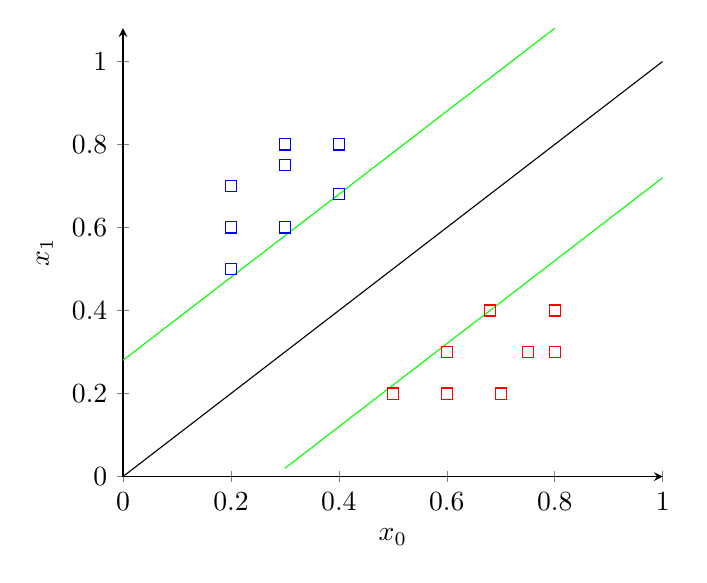
\begin{tikzpicture}
\begin{axis}[
    axis lines = left,
    xlabel = $x_0$,
    ylabel = {$x_1$},
]
\addplot[
    only marks,
    color=blue,
    mark=square,
    ]
    coordinates {
    (0.2,0.7)(0.2,0.5)(0.2,0.6)(0.3,0.8)(0.3,0.6)(0.3,0.75)(0.4,0.8)(0.4,0.68)
    };
\addplot[
    only marks,
    color=red,
    mark=square,
    ]
    coordinates {
    (0.7,0.2)(0.5,0.2)(0.6,0.2)(0.8,0.3)(0.6,0.3)(0.75,0.3)(0.8,0.4)(0.68,0.4)
    };
\addplot [
    domain=0:0.8, 
    samples=100, 
    color=green,
]
{x + 0.28};
\addplot [
    domain=0.3:1, 
    samples=100, 
    color=green,
]
{x - 0.28};
\addplot [
    domain=0:1, 
    samples=100, 
    color=black,
]
{x};
\end{axis}
\end{tikzpicture}
\caption{Plot som viser det optimale hyperplanet i svart og de to støttevektorene i grønt.}
\label{figure:svm}
\end{figure}

Treningen av støttevektormaskiner følger det samme mønsteret som logistisk regresjon, men skiller seg på å ha en annen hypotese og kostnadsfunksjon. Hypotesen er det lineære indreproduktet vi så fra introduksjonen om klassifisering (\ref{eq:hypotese-kompakt}). Kostnadsfunksjonen er enklest forstått gjennom et plot. (\ref{figure:svmcost}) viser de to kostnadsfunksjonene. Dersom klassen $y=1$ ønsker vi at hypotesen $\theta^{T}x \geq 1$. Dersom klassen $y=0$ ønsker vi at hypotesen $\theta^{T}x \leq -1$

\begin{figure}[h!]
\begin{subfigure}{0.5\textwidth}
\centering
\begin{tikzpicture}
\begin{axis}[
    axis lines = center,
    xlabel = $\theta^{T}x$,
    xmin=-2, xmax=2,
    ymin=0, ymax=5,
]
\addplot [
    domain=-2:2, 
    samples=100, 
    color=red,
]
{1 + x};
\addplot [
    domain=-2:-1, 
    samples=100, 
    color=red,
]
{0};
\legend{$cost_0(\theta^{T}x)$}
\end{axis}
\end{tikzpicture}
\end{subfigure}
\begin{subfigure}{0.5\textwidth}
\centering
\begin{tikzpicture}
\begin{axis}[
    axis lines = center,
    xlabel = $\theta^{T}x$,
    xmin=-2, xmax=2,
    ymin=0, ymax=5,
]
%\addlegendentry{$cost_0(\theta^{T}x)$}
\addplot [
    domain=-2:2, 
    samples=100, 
    color=blue,
]
{1 - x};
\addplot [
    domain=1:2, 
    samples=100, 
    color=blue,
]
{0};
\legend{$cost_1(\theta^{T}x)$}
\end{axis}
\end{tikzpicture}
\end{subfigure}
\label{figure:svmcost}
\caption{Plot av støttevektormaskinens kostnadsfunksjoner.}
\end{figure}

Treningen består dermed igjen av å minimere (\ref{eq:svmcost}) med den samme oppdateringsregelen som for logistisk regresjon (\ref{eq:gradient}), men med en ekstra, justerbar parameter $C$ som avgjør hvor mye man ønsker å unngå å feilklassifiere hvert treningseksempel. Med en stor $C$-verdi vil optimaliseringen velge et hyperplan med mindre marginer dersom dette hyperplanet gjør en bedre jobb på å få alle treningsdataene klassifisert riktig. En lav $C$-verdi lar optimaliseringen finne et hyperplan med større marginer, selv dersom dette hyperplanet feilklassifiserer flere datapunkt.

\begin{equation}
J(\theta) = 
    C \sum_{i=1}^{m} y^{(i)}cost_1(h_\theta(x^{(i)})) + (1-y^{(i)})cost_0(h_\theta(x^{(i)}))
\label{eq:svmcost}
\end{equation}

Den typen SVM vi har presentert her er en såkalt lineær SVM eller en SVM uten kjerne. Ved å benytte et såkalt "kernel trick" kan SVM-er også modellere ikke-lineære funksjoner. Dette gjør SVM-er svært fleksible til å håndtere ulike data. I vårt prosjekt er vi kun interessert i de lineære modellene så vi går ikke nærmere inn på dette her. For å håndtere klassifisering av flere klasser benyttes gjerne den samme "en-mot-resten"-strategien som i logistisk regresjon. Denne ender altså opp med å trene $n$ klassemodeller og modellen med det beste resultatet benyttes. I i vårt tilfelle betyr dette at 10 modeller må trenes.
}

\subsection{Brukergrensesnitt}
{\color{blue}
Dagens grafiske brukergrensesnitt har sine røtter i Doug Engelbart's forskning på 60-tallet. Idéene hans ble videreutviklet på Xerox Parc på 70-tallet og ble til slutt en kommersiell suksess gjennom Apple's Macintosh på 80-tallet. Tredve år senere er teknologien videreutviklet, men konseptene bak dagens brukergrensesnitt er omtrent identiske som på den første Macintoshen. REF-ORAMA.

Hva slags programvare trengs i smarte hjem?
God kommunikasjon (gi kommandoer og få feedback), og mulighet til å se hjemmets tilstand.

Referanse til og prat om artikkelen "direct manipulation vs agents".

\subsubsection*{Smarttelefoner og andre touch-skjermer}
Touchskjermer i form av smarttelefoner og nettbrett er nå vidspredte og populære. Dette er et argument for at de også kan representere en interaksjonsform der folk vil være komfortable med å avstandsstyre funksjonalitet i hjemmet. At alle har smarttelefonen med seg gjør også at muligheten til informasjon om og styringsmuligheter av hjemmet er tilstede til en hver tid.

\citet{koskela04} så på tre forskjellige brukergrensesnitt for å styre smarte hjem. De evaluerte bruken av en pc, en tv med fjernkontroll og en mobiltelefon. Resultatene viste at en pc fungerte best som en sentral enhet for å kontrollere aktiviteter som kan planlegges eller bestemmes på forhånd. Dette gjaldt å sette opp automatiseringer, slik som at gardinene skal trekkes for og lysene skal tennes til et visst tidspunkt. Mobiltelefonen ble funnet til å være det beste alternativet for direkte kontroll. Denne studien ble gjort i 2004 og resultatene kan derfor antas å være noe daterte, men resultatet om at en bærbar, mobil enhet var det beste for å direkte kontrollere omgivelsene er nyttig. Dagens smarttelefoner er selvfølgelig kapable til mye mer enn mobiltelefonen fra 2004 og dermed er smarttelefoner og andre touch-skjermer sannsynligvis et godt alternativ for å tilby interaksjon med hjemmet.

\subsubsection*{Omgivelsesskjermer}
\citet{rogers06} skriver at vi bør designe grensesnittene våre proaktivt mennesker og at informasjonskilder, andre mennesker og omgivelsene skal kunne sees og interageres med når det er behov for det. Å ha informasjonskilder tilgjengelig forskjellige steder i hjemmeomgivelsene kan gi nye muligheter for samarbeid mellom mennesker i aktiviteter som omhandler både lek og arbeid.

\emph{Proxemics} foreslås av \citet{greenberg11} som en tilnærming for å gi enheter en mer naturlig oppførsel. De stipulerer at brukere naturlig forventer at når enhetene deres nærmer seg andre enheter eller gjenstander i omgivelsene, øker tilkoblingen og interaksjonsmulighetene forbedres. Om alle finner denne oppførselen naturlig for elektroniske enheter er kanskje diskuterbart, men ideén om at enhetene forandrer seg basert på avstand passer godt inn i modellen for pervasive computing.

Forskjellige interaksjonssoner beskrives av \citet{streitz05}. De omtaler interaksjonssonene omgivende, notifikasjon og interaksjon (figur \ref{commzones}). I den omgivende sonen kan brukeren oppfatte mønstere som vises på en vegg. Veggen sanser avstand til brukeren og viser mønstre ved å tenne et antall små, separate lyskilder. I notifikasjon vil personlige notifiseringsmønstre vises, og i interaksjon vil veggen vise spesielle mønstre og være interagerbar. Bruken av soner gir mulighet til å tilby forskjellige visninger og interaksjoner basert på avstand. Greenberg et al. omtaler fem målbare dimensjoner av \emph{proxemics}: \emph{Avstanden} mellom enheter og brukere virker naturlig, og passer godt inn med interaksjonssonene som er definert. \emph{Retning} gir et mål på vinkelen mellom enheter og brukere. Det finnes allerede enheter som gjør bruk av retning, for eksempel ved å skru seg av når folk ikke ser på dem. \emph{Bevegelse} omfatter forandring i distanse over tid. \emph{Identitet} beskriver en enhet i et gitt detaljnivå. \emph{Plassering} beskriver posisjonen til enheten, for eksempel i hvilket rom og hva konteksten rundt rommet er. \emph{Proxemics} kan i sin helhet være med på å tilby en mer naturlig interaksjon med enhetene våre og kan kanskje være det neste steget for utviklingen av interaksjonsapplikasjoner.
}

Er brukergrensesnitt viktigere enn proaktivitet?
I det forrige kapittelet så vi på hva brukerene ønsker seg. Noen av deres ønsker kan være vanskelig å implementere uten å bryte andre ønsker, som at systemet skal forstå konteksten i omgivelsene uten å være overvåkende. Uansett, det viktigste for de spurte gruppene var å selv være i kontroll av et systemet som var enkelt å bruke og som ga muligheter til å styre diverse deler av huset, inkludert elektriske apparater, hvitevarer, hjemmeunderholdning, lys og varme. Alt i alt er det kanskje viktigere for vanlige brukere at det tilbys gode styringsmuligheter, enn at systemet er proaktivt?

I en kontroversiell artikkel fra 2006 påpeker \citet{rogers06} at vi ennå ikke gjør "smart" på en god måte, nettopp fordi det involverer å løse svært vanskelige problemer innen kunstig intelligens . Tre områder har vært fokuset for \emph{pervasive/ubiquitous computing}: kontekstbevissthet, omgivelser som responderer til menneskelig tilstedeværelse og overvåking. Disse problemene kan på flere måter sees på som vanskeligere å løse enn det å skape et kunstig menneske. Forskningsmiljøet har møtt spesielt store problemer med den store variasjon i hva folk gjør, hvilke motiver de har, når de gjør det og hvordan de gjør det. Konteksten rundt folks dagligdagse liv er svært subtil og det i en mye større grad enn kontekstteorier har fått oss til å tro. Dette gjør det vanskelig, om ikke umulig, å implementere kontekst slik at det kan dras nyttige spådommer om hva mennesker føler, hva de ønsker eller hva de trenger i et gitt øyeblikk. Det finnes også etiske og sosiale bekymringer. I kapittel en nevnte vi Mark Weiser's drøm om \emph{calm computing}, der omgivelsene er gjennomtrengt med teknologi som støtter opp våre liv og gjør dem så komfortable som mulig. La oss si at Weisers drøm blir en virkelighet. Er dette en tilværelse vi ønsker å leve i? Bør de menneskelige kognitive prosessene druknes med en assistert levetilværelse?

Rogers foreslår en alternativ agenda. Hun argumenterer for et skifte fra proaktiv databehandling to proaktiv mennesker. Allestedsnærværende teknologier bør designes slik at brukere kan interagere med dem mer aktivt. I stedet for \emph{calm living} bør vi ønske \emph{engaged living}. Mennesker, i stedet for maskiner, bør ta initiativet til å være konstruktive, kreative og engasjere i interaksjoner. I stedet for å pakke omgivelsene med all slags forsvinnende teknologi, bør vi tenke på teknologien som et sett med verktøy og overflater som er mobile og tilrettelegger for samarbeid. Informasjonskilder, andre mennesker og omgivelsene kan sees og interageres med når det er behov for det. Videre forskning bør ha fokuset at datamaskiner representerer verktøy, enheter og systemer som kan utvide og engasjere folk i deres aktiviteter og sysler. Vi må få tilbake gleden med interaksjon på innovative måter.

{\color{blue}


\subsubsection*{Tale}
{\color{blue}
Kort intro til drømmen med tale. Drømmen om kontinuerlig talekommunikasjon med datamaskinene/hjemmet. Et system som skal forstå naturlig tale må kunne gjenkjenne og skille tusenvis av ord i forskjellige kombinasjoner, i forskjellige språk og uttaler. Fagområdet som jobber med dette problemet heter "Naturlig språk-prosessering". 

Fra AIMA
Talegjenkjenning er å identifisere en sekvens av ord ut i fra et akustisk signal. Det har blitt en av teknikkene fra KI som har blitt populært og vidspredt. Talegjenkjenning benyttes daglig av brukere verden over for å gi navigasjonsinstrukser til bilene sine, gjøre søk på nettet eller å skrive gjennom diktasjon. Tale er en attraktivt interaksjonsform i alle tilfeller der brukeren kan ha bruk for å gjøre andre ting med hendene, eller der han ikke har muligheten til å bruke dem.

Det er ingen enkel oppgave å gjenkjenne tale. Lydene brukeren lager inneholder ofte støy og det finnes en rekke setninger som høres like ut når de sies fort. Når vi skriver setninger er det mellomrom mellom ordene, men i tale er det setninger som uttales uten pause mellom ordene. Det er også mange ord som uttales likt, men skrives forskjellig og har forskjellig betydning avhengig av kontekst.

Talegjenkjenning handler om å finne den mest sannsynlige sekvensen av ord. Denne mest sannsynlige sekvensen kan kalkuleres ved bruk av Bayes' regel:

{\color{red}bayes} argmax P(word|sound) er lik argmax P(sound|word)P(word)
P(sound|word) er en akustitisk modell; en beskrivelse av lydene til ord. P(word) er språkmodellen, som sier noe om den foregående sannsynligheten til hver uttale. For eksempel kan språkmodellen si at "Spise iskrem" er 1000 ganger så sannsynlig som "Grise iskrem".

Denne framgangsmåten ble kalt "noisy channel model" av Claude Shannon (1948) {\color{red}ref}, som viste at uavhengig av hvor bråkete kanalen som fører signalet er, så kan et orginalt signal bli forstått med en lav feilmargin dersom det orginale signalet enkodes på en tilstrekkelig overflødig måte.

De fleste talegjenkjenningssystemene i dag benytter en språkmodell etter Markov-antakelsen, altså at den nåværende tilstanden, Word1, avhenger kun av et fiksert antall foregående tilstander, og Word1 er representert som en enkelt tilfeldig variabel bestpende av et begrenset sett med verdier, hvilket gjør den til en Hidden Markov Model (HMM). Altså kan talegjenkjenning løses ved å anvende HMM-metodologien.

Fra CMUSphinx
Tale virker enkelt å forstå: det er bygget opp av ord og hvert ord består av fonemer. I virkeligheten er det desverre svært annerledes. Tale er en dynamisk prosess uten klare skiller mellom ulike deler. De moderne måtene å beskrive tale på er i større eller mindre grad basert på sannsynligheter. Denne måten å se situasjonen på lar oss forstå at talegjenkjenning aldri vil være 100\% korrekt.

Tale er en kontinuerlig strøm av audio der relativt stabile tilstander blander seg med dynamiske tilstander. I denne strømmen av tilstander kan man forsøke å definere klasser av lyder, kalt fonemer. De akustiske egenskapene til bølgeformen til et fonem kan variere kraftig avhengig av faktorer som omgivelseslyder, hvem som taler og hvordan denne kilden taler. Disse variasjonene kan gjøre at fonemer oppfattes svært annerledes ut enn det de skulle representere. 
En strategi for å hjelpe mot disse problemene er å innse at de viktigste datapunktene er i overgangene mellom ord. Utviklere benytter ofte tre regioner i strømmen for å gjenkjenne et ord: den første delen avhenger av det foregående fonemet, midtpartiet er relativt stabilt, og den tredje delen avhenger av det følgende fonemet. Fonemer bygger subord-enheter, som stavelser. Stavelser kan være nyttige å modellere etter og de er kjent som "reduction-stable entities". Når tale utføres raskt vil fonemer ofte være annerledes, men stavelser forblir de samme. Flere subord danner ord. Ord er viktig i talegjenkjenning fordi de begrenser kombinasjonen av fonemer. Dersom det er 40 fonemer og et gjennomsnittlig ord har 7 fonemer finnes det 40 opphøyd i 7 mulige ord. Heldigvis benytter de fleste mennesker omtrent 10000 ord til daglig, hvilket gjør talegjenkjenning mer håndterlig.

Ord, sammen med andre ikke-lingvistiske lyder (som pust, hoste, pauselyder), danner ytringer. Ytringer er separate lyder mellom pauser. 

Den vanlige måten å gjenkjenne tale på er følgende: man mottar en bølgeform, splitter den inn i ytringer delt av stillhet og forsøker så å gjenkjenne hva som blir sagt i hver ytring. For å gjøre dette tar vi alle mulige kombinasjoner av ord og forsøker å matche dem med lyden. Vi velger så den kombinasjonen som passer best.

Tale modelleres gjerne med en Hidden Markov Model (HMM). Modellen beskriver en sekvens av tilstander der overgangen er gitt av en sannsynlighet. Det er en generell modell som kan beskrive alle sekvensielle prosesser og den har vist seg å være spesielt praktisk for å dekode tale.

Tre modeller benyttes i talegjenkjenning for å matche ord med lyd. En akustisk modell, en ordbok og en språkmodell. Den akustiske modellen holder akustiske egenskaper for kombinasjoner av fonemer. En enkel fonetisk ordbok knytter ord med fonemer. Denne naive varianten er ikke veldig effektiv ettersom den ikke tar større hensyn til forskjellige uttaler, men den fungerer som regel i praksis. Maskinlæring kan benyttes her for å lære langt mer nyanserte sammenhenger. En språkmodell brukes for å innsnevre søket etter det passende ordet. Den definerer hvilke ord som kan følge etter det foregående gjenkjente ordet og hjelper dermed med å fjerne ord som ikke er sannsynlige. De fleste språkmodeller er n-gram modeller, som inneholder statistikk over ord-sekvenser, eller finite-state-modeller, som definerer talesekvenser av finite-state-automation med vekting. For å oppnå en god presisjon må språkmodellen utføre en god jobb på å begrense søkeområdet for mulige ord. Den må altså være svært god på å gjette det neste ordet. En språkmodell begrenser som regel vokabularet til ordene den inneholder. Dette skaper problemer med navn-gjenkjenning. Derfor kan en språkmodell også inneholde mindre deler, som subord eller til og med fonemer. Søkeområdet øker dersom disse introduseres og leder som regel til svakere presisjon enn med en ord-basert språkmodell.  

Prosjekter som benytter tale (google, apple, samsung, ..).
}

\subsubsection*{Gester}
{\color{blue}
En annen interaksjonsform det forskes på er gester. Dette er nok et forsøk på å tilby en mer naturlig interaksjon med datamaskinen. Kroppsspråket er tross alt en stor del av mellommenneskelig kommunikasjon, så hvorfor ikke forsøke å utvide det til kommunikasjon mellom menneske og maskin.

Papers fra IUI som benytter gester (multimodalitet).

Tilnærmingen i disse prosjektene er kameraer som måler farger og dybde, samt avanserte algoritmer for datasyn. Sammen kan disse prosessere informasjonen og danne grunnlaget for et system som kan gjenkjenne kompliserte gester.

\citet{homeos} omtaler en prosjektgruppe som utvidet HomeOS-systemet til å forstå gester, ved bruk av Kinect-kameraet.

Paper fra CHI 2014..
}

\subsubsection*{Multimodalitet}
{\color{blue}
Multimodalitet i forbindelse med datasystemer betyr å forbedre forståelsen gjennom en kombinasjon av flere input-kanaler. Meningen er å forbedre systemets nøyaktighet i å oppdage og forstå input-signaler, kanskje spesielt når dataene kommer på forskjellige og ikke-overlappende former. \citet{placelab05} og \emph{Placelab}-prosjektet er et bra eksempel på å kombinere video og audio for å bedre nøyaktigheten i å detektere menneskelig aktivitet. Faktisk oppdager vi at mange prosjekter gjør bruk av kombinasjoner av diverse sensorteknologier for å danne et rikere tilstandsbilde og for å forbedre nøyaktigheten. \citet{desilva12} nevner et prosjekt der en robot følger et menneske gjennom multimodale teknikker. Roboten har en visuell input og er trent gjennom et kunstig nevralt nettverk til å skille hudfarge fra omgivelsene og dermed identifisere mennesket. I tillegg benytter roboten seg av en sonarskanner samt taktile sensorer for å beregne avstanden til mennesket.

Prosjekter fra IUI-pensum.

}

\subsubsection*{Brain Interfaces \& Annet}
{\color{blue}
Kort om hva det er, ref IUI-pensum.

The conventional means of interfacing the brain to the world (ie, the body) was developed over millions of years, and works splendidly. Today's computer interfaces were hacked together over a few decades. If there's a mismatch between our bodies and our computers, don't you suspect that the fault might lie on the computer's side? Perhaps our computers should be adapted to fit our bodies, instead of blithely bypassing our bodies entirely.

We've almost given up on the body already. We sit at a desk while working, and sit on a couch while playing, and even sit while transporting ourselves between the two. We've had to invent this peculiar concept of artificial "exercise" to keep our bodies from atrophying altogether.

It won't be long before almost every one of our daily activities is mediated by a "computer" of some sort. If these computers are not part of the physical environment, if they bypass the body, then we've just created a future where people can and will spend their lives completely immobile.

Why do you want this future? Why would this be a good thing?
}


